\section{Metodologia}

O modelo para reconfiguração do sistema de distribuição de energia elétrica, abordado nesse projeto, foi implementado em linguagem de modelagem matemática.

\subsection{Introdução a Linguagem de Programação Matemática}

%Editar essa parte - Colocar mais para baixo e colocar uma
%introdução de linguagem de modelagem matematica
O AMPL é uma linguagem procedural de modelagem algébrica cuja função é descrever e resolver problemas a partir do seu modelo matemático. 
A linguagem fora desenvolvida nos \emph{Bell Labs} por Robert Fourer, David Gay e Brian Kernighan com o intuito de ajudar as pessoas a comunicar modelos de otimização para sistemas de computação, aproveitando o poder e a conveniência de formulações algébricas familiares \cite{ampl}. 

Possui, atualmente, suporte para uma grande diversidade de \textit{solvers} tanto comerciais quanto código aberto.

%%%%%%%%%%%%%%%%%%%%%%%%%%%%%

Os benefícios envolvendo o uso da linguagem estão relacionados ao fato de ser possível lidar com modelos algébricos, complexos e de larga escala, de maneira fácil e intuitiva que serão traduzidos em dados que podem ser processados por programas solucionadores.

Exemplos de problemas como descritos em \cite{Fourer2003AMPLProgramming} são:

\begin{itemize}
    \item Modelo de transporte \textit{multicommodity};
    
    \item Modelo de produção multiperiódico;
    
    \item Modelo de produção e transporte.
\end{itemize}

Os exemplos citados anteriormente são apenas uma parcela de uma infinidade de problemas de programação de larga escala.


A estrutura básica de um modelo em AMPL é da seguinte forma como mostrada em \cite{taha2008pesquisa}:

\begin{table}[H]
    \centering
    \caption{Estrutura de um modelo em AMPL}
    \begin{tabular}{|c|l|}
        \hline
        \multirow{4}{*}{Representação algébrica} & Definição dos conjuntos\\ & Definição dos parâmetros\\ & Definição das variáveis\\ & Representação do modelo\\ \hline
        
        
        \multirow{3}{*}{Implementação do modelo} & Dados de entrada\\ & Solução do modelo\\ & Apresentação dos resultados\\
        \hline
    \end{tabular}
    \label{tab:estrut_AMPL}
\end{table}
    
    \vspace{8pt}
    
A vantagem desse arranjo é que o mesmo modelo algébrico pode ser usado para resolver um problema de mesma natureza mas de tamanho diferente.



\subsection{\emph{Solvers}}

\emph{Solvers}, como dito anteriormente, são programas que tem como finalidade buscar uma solução ótima baseada em um conjunto de parâmetros e podem ser tanto comerciais quanto constituídos de código aberto.
Ambas as categorias podem resolver determinados problemas de acordo com a natureza do sistema.


Um exemplo de \emph{solver} usado para resolver problemas de otimização linear e quadrática em variáveis contínuas e inteiras é o CEPLEX, solver comercial baseado essencialmente em linguagem C cuja licença pertence à empresa IBM.
O suporte é fornecido para soluções de problemas quadráticos convexos, não convexos e restrições quadráticas convexas \cite{amplCEPLEX}. Os algoritmos usados são:

\begin{itemize}
    \item Problemas contínuos: primal e dual simplex, ponto interior;
    
    \item Problemas de números inteiros: \textit{branch and bound}, heurísticas de viabilidade e geradores de corte.
\end{itemize}

Outro exemplo de \emph{solver}, esse utilizado para solução de problemas de otimização não lineares, é o KNITRO.
O KNITRO é um pacote de programas em C para resolver otimização não linear e não linear inteiro misto, uma particularidade do software foi a grande atenção dada ao desempenho dos algoritmos KNITRO em classes mais simples de problemas, como sistemas de equações não-lineares e problemas irrestritos, uma vez que essas tarefas são cruciais na solução de problemas de programação não linear \cite{Byrd2006Knitro:Optimization}.
Segundo a Artelys, empresa responsável pelo software, o mesmo conta com os seguintes recursos para a solução de problemas de otimização, mostrados em \cite{knitroweb}:

\begin{itemize}
    \item Quatro algoritmos de ponto ativo/conjunto interno para problemas PNL;
    
    \item Três algoritmos para otimização discretas de problemas PNLIM;
    
    \item restrições de complementaridade para problemas de equilíbrio.
\end{itemize}

A entrada de um \emph{solver} para solução de problemas PNLIM, pode ser tomado como exemplo o manual disponível no NEOS-server como mostrado em \cite{neosguide}.

\begin{tcolorbox}[colback=white!10,title =\textbf{Conceitos básicos }]
    \begin{minipage}{\dimexpr\textwidth-\shadowsize-2\fboxrule-2\fboxsep-8pt}
    
    \begin{center}
        Min: $f(x,y)$   
    \end{center}

    \hspace{2cm}Sujeito a: 

    \begin{align*}
        c_{i}(x,y) = 0 \qquad \forall i&\in E\\
        c_{i}(x,y) \leq 0 \qquad \forall i&\in I\\
        x \qquad &\in X\\
        y \qquad &\in Y \quad \text{inteiro}
    \end{align*}
    \end{minipage}
    
    \vspace{1cm}
    
    Onde cada $c_{i}(x,y)$ é um mapeamento de $R^n \to R$, e $E$ e $I$ são conjuntos de índices para restrições de igualdades e desigualdades respectivamente. Tipicamente, as funções $f$ e $c_{i}$ têm algumas propriedades de suavidade, isto é, uma ou duas vezes continuamente diferenciáveis.
\end{tcolorbox}

\subsection{Hipóteses e definições da formulação do problema}

\begin{figure}[H]
    \centering
    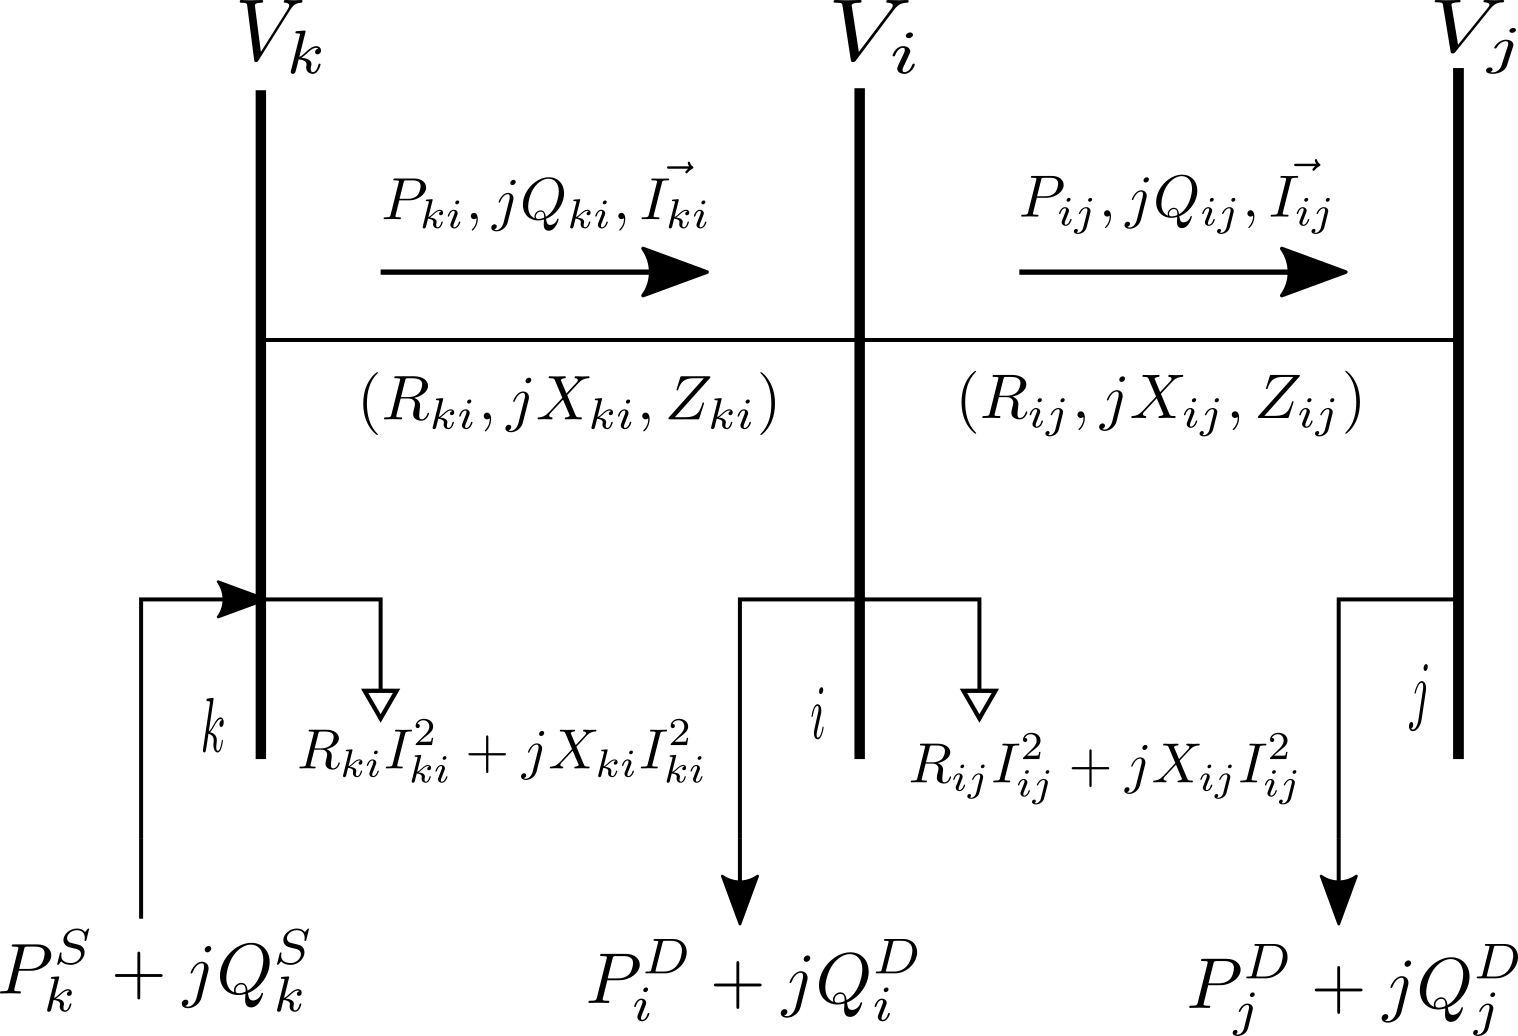
\includegraphics[width=0.7\textwidth]{3_Methodology/diagrama_nos.png}:
    \caption{Sistema de distribuição (Representação em barras)}
    \label{fig:SDR}
\end{figure}

Hipóteses adotadas:
Visando representar o funcionamento em regime permanente de um sistema de distribuição de energia, são feitas as seguintes hipóteses (comumente usadas nas formulações de varredura de fluxo de carga \cite{Shirmohammadi1988ANetworks} e mostradas na figura \ref{fig:SDR}):

\begin{itemize}
    \item As demandas das cargas na rede de distribuição são representadas como potência ativa e reativas contantes;

    \item O sistema é balanceado e representado pelo seu equivalente monofásico;
    
    \item As perdas de potência ativa e reativa no circuito \textit{ij} estão concentradas no nó \textit{i};
    
    \item As chaves são representadas como curtos circuitos de impedância nula.
\end{itemize}

\subsection{Modelo de otimização}

O modelo de otimização para RSD interpretado pelo AMPL possui a seguinte forma:

\begin{tcolorbox}[colback=white!10,title =\textbf{Modelo de um problema de otimização para RDS}]
    \begin{minipage}{\dimexpr\textwidth-\shadowsize-2\fboxrule-2\fboxsep-8pt}
    
    \begin{center}
        Minimizar: Função objetivo        
    \end{center}

    \hspace{2cm}Sujeito a:

    \begin{center}
        Restrições físicas\\
        Restrições operativas\\
    \end{center}
    \end{minipage}
\end{tcolorbox}


As restrições do problema devem ser tais que modelem as leis da física que regem um sistema de distribuição de energia elétrica e as faixas com as quais essas grandezas podem operar ao longo da rede.
Para isso define-se dois conjuntos de restrições, restrições físicas e restrições operativas.